%%
%% This is file `sample-sigconf.tex',
%% generated with the docstrip utility.
%%
%% The original source files were:
%%
%% samples.dtx  (with options: `sigconf')
%% 
%% IMPORTANT NOTICE:
%% 
%% For the copyright see the source file.
%% 
%% Any modified versions of this file must be renamed
%% with new filenames distinct from sample-sigconf.tex.
%% 
%% For distribution of the original source see the terms
%% for copying and modification in the file samples.dtx.
%% 
%% This generated file may be distributed as long as the
%% original source files, as listed above, are part of the
%% same distribution. (The sources need not necessarily be
%% in the same archive or directory.)
%%
%%
%% Commands for TeXCount
%TC:macro \cite [option:text,text]
%TC:macro \citep [option:text,text]
%TC:macro \citet [option:text,text]
%TC:envir table 0 1
%TC:envir table* 0 1
%TC:envir tabular [ignore] word
%TC:envir displaymath 0 word
%TC:envir math 0 word
%TC:envir comment 0 0
%%
%%
%% The first command in your LaTeX source must be the \documentclass command.
\documentclass[sigconf]{acmart}

\usepackage{pgfplotstable}

\setlength {\marginparwidth }{2cm}
\usepackage[colorinlistoftodos]{todonotes}
\usepackage{tabularx}
\usepackage{pgfplots}
\pgfplotsset{compat=1.17}
\usetikzlibrary{calc}

%%
%% \BibTeX command to typeset BibTeX logo in the docs
\AtBeginDocument{%
  \providecommand\BibTeX{{%
    \normalfont B\kern-0.5em{\scshape i\kern-0.25em b}\kern-0.8em\TeX}}}

%% Rights management information.  This information is sent to you
%% when you complete the rights form.  These commands have SAMPLE
%% values in them; it is your responsibility as an author to replace
%% the commands and values with those provided to you when you
%% complete the rights form.
\setcopyright{acmcopyright}
\copyrightyear{2021}
\acmYear{2021}
\acmDOI{}

%% These commands are for a PROCEEDINGS abstract or paper.
\acmConference[K-Cap '21]{K-Cap '21: The Eleventh International Conference on Knowledge Capture}{December 02--03, 2021}{Virtual Conference}


%%
%% Submission ID.
%% Use this when submitting an article to a sponsored event. You'll
%% receive a unique submission ID from the organizers
%% of the event, and this ID should be used as the parameter to this command.
%%\acmSubmissionID{123-A56-BU3}

%%
%% The majority of ACM publications use numbered citations and
%% references.  The command \citestyle{authoryear} switches to the
%% "author year" style.
%%
%% If you are preparing content for an event
%% sponsored by ACM SIGGRAPH, you must use the "author year" style of
%% citations and references.
%% Uncommenting
%% the next command will enable that style.
%%\citestyle{acmauthoryear}

%%
%% end of the preamble, start of the body of the document source.
\begin{document}

%%
%% The "title" command has an optional parameter,
%% allowing the author to define a "short title" to be used in page headers.
\title{OntoFlow : Easy Ontology Development Workflows for Non-technical Domain Experts}

%%
%% The "author" command and its associated commands are used to define
%% the authors and their affiliations.
%% Of note is the shared affiliation of the first two authors, and the
%% "authornote" and "authornotemark" commands
%% used to denote shared contribution to the research.
\author{Gordian Dziwis}
\authornote{}
\email{dziwis@infai.org}
\author{Lisa Wenige}
\authornotemark[1]
\email{wenige@infai.org}
\author{Lars-Peter Meyer}
\authornotemark[1]
\email{meyer@infai.org}
\affiliation{%
  \institution{Institute for Applied Informatics}
  \streetaddress{Goerdelerring 9}
  \city{Leipzig}
  \state{Saxony}
  \country{Germany}
  \postcode{04177}
}

%%
%% By default, the full list of authors will be used in the page
%% headers. Often, this list is too long, and will overlap
%% other information printed in the page headers. This command allows
%% the author to define a more concise list
%% of authors' names for this purpose.
\renewcommand{\shortauthors}{Dziwis and Wenige et al.}

%%
%% The abstract is a short summary of the work to be presented in the
%% article.
\begin{abstract}
  For many years, the development of widely applicable and high quality ontologies has been an ongoing research topic. Among the many challenges, the lack of integrated development environments for non-technical domain experts has been one of the most pressing research challenges. But while the participation of domain experts is vital for the applicability of ontologies, there are hardly any software tools available that facilitate their active engagement. We present a solution that addresses this research gap by automating the ontology development process with the help of a workflow engine. We define a pipeline that facilitates ontology implementation, serialization, documentation and testing within the scope of a seamless automatic routine than can be easily triggered by an ontology laymen with basic knowledge of bash usage. Thus, the processing pipeline takes care of most of the operations that usually have to be taken care of by an ontology or software engineer. We demonstrate the applicability of our approach for a wide range of ontologies and provide additional results on the quality level of ontologies throughout the Semantic Web landscape.
\end{abstract}

%%
%% The code below is generated by the tool at http://dl.acm.org/ccs.cfm.
%% Please copy and paste the code instead of the example below.
%%
\begin{CCSXML}
  <ccs2012>
  <concept>
  <concept_id>10010520.10010553.10010562</concept_id>
  <concept_desc>Computer systems organization~Embedded systems</concept_desc>
  <concept_significance>500</concept_significance>
  </concept>
  <concept>
  <concept_id>10010520.10010575.10010755</concept_id>
  <concept_desc>Computer systems organization~Redundancy</concept_desc>
  <concept_significance>300</concept_significance>
  </concept>
  <concept>
  <concept_id>10010520.10010553.10010554</concept_id>
  <concept_desc>Computer systems organization~Robotics</concept_desc>
  <concept_significance>100</concept_significance>
  </concept>
  <concept>
  <concept_id>10003033.10003083.10003095</concept_id>
  <concept_desc>Networks~Network reliability</concept_desc>
  <concept_significance>100</concept_significance>
  </concept>
  </ccs2012>
\end{CCSXML}

\ccsdesc[500]{Computer systems organization~Embedded systems}
\ccsdesc[300]{Computer systems organization~Redundancy}
\ccsdesc{Computer systems organization~Robotics}
\ccsdesc[100]{Networks~Network reliability}

%%
%% Keywords. The author(s) should pick words that accurately describe
%% the work being presented. Separate the keywords with commas.
\keywords{ontologies, workflows, IDE, quality assurance}

%%
%% This command processes the author and affiliation and title
%% information and builds the first part of the formatted document.
\maketitle

\section{Introduction}
keywords:
\begin{itemize}
  \item no standard toolstack in the Semantic Web community => containerisierung 
  \item usability

  \item take idea of CI pipeline to ontology engineering

  \item we need modern tools for ontology engineering to help a broader range of participants including non-technical domain experts
\end{itemize}

Currently there is quite a lot of effort taken to use the gain from semantic modeling in different areas. This includes biomedicine, finance, engineering, law, and cultural heritage [Tudorache2020] \todo{doi 10.3233/SW-190382} . But although there is much to get from utilizing and engineering ontologies, modern ontology engineering involves still quite a lot of labour intensive tasks to handle the diverse tools for ingestion of domain knowledge, testing and documenting. In addition to that many of the tools available are difficult to handle for domain experts without IT or semantic web background.

In software engineering automation with workflow pipelines step in here, especially with continuous integration and deployment (CI/CD) pipelines \todo{Humble2010 ISBN 9780321670229}. This eases the process from basic checks over compilation and testing to deploying and removes the need for time consuming repetitive and error prone manual work. For handling the diverse many software tools, containerization can step in. The use of Open Containers Initiative (OCI) Containers and Container Images helps with bundling and updating software tools with all their dependencies.

\section{Related Work}
Continuous development and integration strategies have become an indispensable part of modern software engineering.
They largely consist of clean up operations, compilation of executables, application of automated tests, and the deployment of the finished application, including generation of appropriate documentation if necessary. Part of these processes is the continuous checking of any updates/ new versions as well as the triggering of troubleshooting activities if problems occur \cite{fowler}.
This ensures that software solutions are always up-to-date, that applications meet predefined quality standards and rely on stable software artifacts.\\
Likewise, in the wake of ever-growing data volumes and increased relevance of data-driven applications, effective mechanisms to control the quality-assured publication of data products have become important requirements for IT operations. Processes that follow Continuous Integration (CI) principles are equally applicable when the production of data artifacts in collaborative environments should be made more efficient. The knowledge graph community has been one of the first to adopt DevOps best practices for datasets since it heavily relies on high quality data schemas and reproducible workflows for data conversion, integration and fusion. In this line of research, several authors have proposed automated data pipelines that not only take care of data transformation but also apply quality assurance operations and automatic procedures for data publication and effective description of data artifacts
\cite{cirulli, klimek, kucera, meissner, rojas, roman, stadler, dataid}. Typically, CI mechanisms for data collections involve operations such as crawling, linking, or data transformation. These processes are usually executed automatically and, aside from the effort of creating specifications for data conversion, are little interrupted by user interactions and manual intervention. If people work with appropriate software tools in this context, they are mostly data scientists or software engineers.\\
This modus operandi differs from the determining factors in ontology development processes. The creation of an ontology usually involves several experts with diverse backgrounds and different levels of technical expertise. Therefore, an effective ontology development environment/pipeline has to foster collaboration as well as provide a graphical editor in order to effectively support development processes. By this means, even domain experts with little IT expertise can actively take part in the creation of ontologies.\\
Ontology editors such as Protégé \cite{protege}, Vocol \cite{halilaj} or WebVOWL \cite{lohmann} are already established software tools for ontology development and visualisation. Meanwhile, other applications in this area focus more on aspects of collaborative and version-based storage of ontologies so that changes can be managed decentrally and tracked over time. Software tools, such as Ontoology \cite{alobaid} or the QuitStore \cite{arndt} provide solutions for these kinds of requirements.\\
Other tools, such as Oops! focus more on the aspect of quality assurance \cite{poveda} while general purpose RDF data testing suites, such as RDFUnit \cite{rdfunit} or pySHACL\footnote{\url{https://github.com/RDFLib/pySHACL}} can be equally applied for ontology testing. Just as important as quality assurance of ontologies is documentation prepared for end users in a form understandable by users. Software applications that automatically generate ontology documentations are WIDOCO \cite{widoco}, LODE \cite{lode} or pyLODE\footnote{\url{https://github.com/RDFLib/pyLODE}}. They create a HTML representation from ontologies in standard RDF serialization formats.\\
But although software applications are already available that support collaborative ontology development processes and also automate them in parts, there is a lack of approaches as to how these processes can be linked in the sense of a CI pipeline while at the same time ensuring that laymen can actively participate in development through making changes and triggering ontology updates.
\todo{https://www.nature.com/articles/s41587-020-0439-x}

\section{Ontology Development Workflow}
\label{sec:ontoflow}
\subsection{Requirements}

% Please add the following required packages to your document preamble:
% \usepackage{booktabs}
% \usepackage{multirow}
\begin{table*}[htb]
\begin{tabular}{@{}lll@{}}
\toprule
Main Requirement &
  Sub-Requirement &
  Explanation \\ \midrule
\textbf{RQ1 ODP Automation} &
  RQ1.1 Ontology serialization &
  \begin{tabular}[l]{@{}l@{}}Ontology artifacts can be automatically \\ serialized in common RDF formats \\ (e.g., RDF/XML, Turtle or NTRIPLES\end{tabular} \\\\
 & 
  RQ1.2 Ontology Validation &
  \begin{tabular}[l]{@{}l@{}}Automatic testing of ontology artifacts\\ is integrated\end{tabular} \\\\
 &
  RQ1.3 Ontology Postprocessing &
  \begin{tabular}[l]{@{}l@{}}Intgrating automatic postprocessing \\ operations, such as updating meta-information, \\ version control or diff detection\end{tabular} \\\\
 &
  \begin{tabular}[l]{@{}l@{}}RQ1.4 Ontology Publication and \\ Documentation\end{tabular} &
  \begin{tabular}[l]{@{}l@{}}Automatic deployment of ontology artifacts \\ (serialization and HTML documentation) to a server\end{tabular} \\\\
\textbf{RQ2 High (Re-)Usability} &
  RQ2.1 GUI support &
  \begin{tabular}[l]{@{}l@{}}Support of ontology modelling through \\ a GUI\end{tabular} \\\\
 &
  \begin{tabular}[c]{@{}l@{}}RQ2.2 Easy execution ontology workflows\end{tabular} &
  \begin{tabular}[c]{@{}l@{}}Domain experts (with little to no IT background)\\ should be able to trigger ontology workflows \\ execute and modify them easily \end{tabular} \\\\
 & 
 \begin{tabular}[c]{@{}l@{}}RQ2.3 Fast execution of ontology workflows\end{tabular} &
  \begin{tabular}[c]{@{}l@{}}It should be possible to quickly generate an ontology, \\ validate it and create its documentations\end{tabular} \\\\
\hline
\end{tabular}
\caption{Requirements for OntoFlow}
\label{tab:req}
\end{table*}

The goal of OntoFlow is the best possible optimization and automation of ontology development processes which typically currently involve a great number of labor-intensive tasks, such as modeling, serialization, updating testing and documentation. Due to the fact that such development processes are carried out by several stakeholders, the workflow environment should foster a collaborative and decentralized way of working.\\
Since the development of ontologies often involves domain experts who have only limited expertise in the field of software and data engineering, OntoFlow should provide a GUI for editing the ontology, while automating the most common tasks (e.g., bash scripting and git interaction) in the background. Due to the limited IT experience of some of the involved stakeholders, it is also vital that workflows can be triggered without in-depth technical understanding of software development or semantic technologies. Reducing the amount of necessary skills for the domain expert is critical, because generally ontology development is a one time job for them. A reusable ontology workflow setup directed at domain experts helps avoiding costs for learning the involved technologies and setting up a development and hosting infrastructure (e.g., running a web server for publishing the ontology and documentation) which - apart from working time - can incur further costs for licences and hardware. Because there is no established methodology for ontology development and it happens in diverse environments, OntoFlow must be flexible and facilitate easy modifications to accommodate for different needs.\\
Table \ref{tab:req} gives an overview of the requirements detailed in the above sections.

\subsection{Workflow Structure}

\begin{figure}[ht]
  \centering
  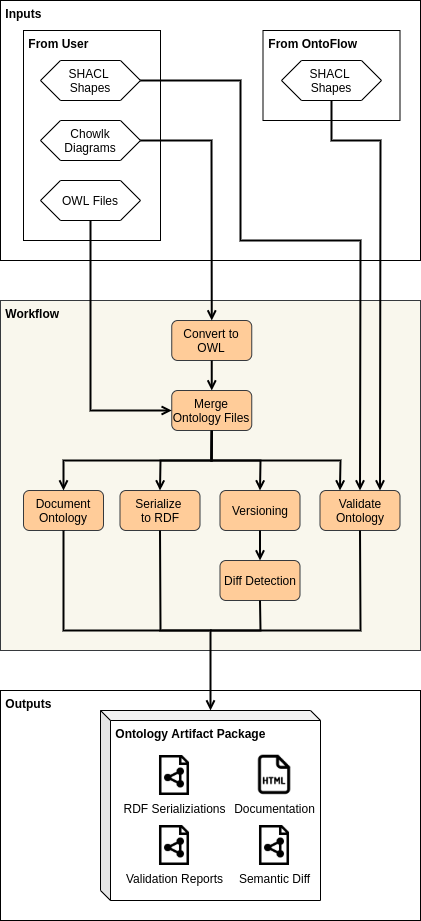
\includegraphics[scale = 0.4]{workflow.png}
  \caption{OntoFlow Workflow}
  \label{fig:workflow}
\end{figure}

Inputs for the workflow are provided by the ontology developer and OntoFlow.
The ontology developer provides ontology diagrams, OWL files and validation shapes.
A ontology diagram is visual representation of an ontology.
The OWL files define ontologies with the Web Ontology Language (OWL) and are serialized as a RDF file.
The ontology is validated against the validation shapes to ensure satisfies a set of conditions.
A set of validation shapes, which test the ontology for formalizable best practice, are supplied by OntoFlow.\footnote{https://gitlab.com/kupferdigital/ontoflow/-/tree/master/shacl}

First process step is the transformation of the ontology diagrams to OWL files and merging those with those OWL files provided by the user.
The resulting ontology is the input for the following parallel processing steps.
A HTML documentation is generated, describing the ontology's metadata, classes and properties.
The ontology is serialized into multiple RDF formats.
In the ontology validation process step, the ontology is validated against the user's and OntoFlow's shapes.
OntoFlow picks up the `owl:priorVersion` property and detects semantic differences to the previous version. This gives an overview which classes changed in the current version compared to the prior version.

The serializations, documentation, validation reports and the semantic differences compose the Ontology Artifact Package.

\subsection{Implementation and Architecture}

\begin{figure}[ht]
  \centering
  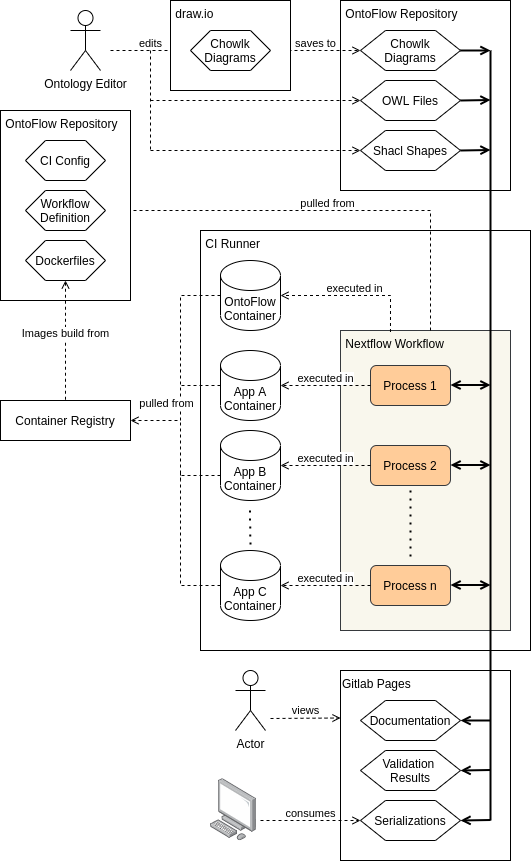
\includegraphics[scale=0.4]{architecture.png}
  \caption{OntoFlow Architecture}
  \label{fig:architecture}
\end{figure}

The architectural model for OntoFlow is a pipeline consisting of processes where each process takes inputs, transform the inputs and outputs the results.
Inputs and output from the processes are interconnected.
Each process's transformation is applied to the inputs by application program with a command-line interface.
All applications are containerised and the container images are defined by an definition file.
A workflow engine manages the containers' life cycle and executes the applications and pipes the inputs and outputs between the processes.
The pipeline process steps, with their corresponding commands to execute, their executing containers, inputs and outputs are defined in a workflow definition file.
Each application container is based on a image for which a configuration file exists.
There is a container for OntoFlow itself, which has all the dependencies necessary for running the workflow engine.
The images are hosted in a container registry.
A continuous integration script builds the images and pushes them to the container registry.
Those file are managed inside a version control system.

The diagrams and files defining the ontology are also hosted in a repository.
OntoFlow provides a continuous integration script, which triggers when a change in the ontology repository occurs.
When triggered the OntoFlow container is started with ontology repository mounted.
Inside the container the workflow engine starts the workflow with the files from the ontology repository and OntoFlow's validation shapes as inputs.
Each process step is then executed in its defined application container.
The final outputs are deployed to their target environment.


The pipeline was implemented as a Nextflow workflow and Docker was chosen as the container engine.
For each tool used in a process step a Docker image was created, if not one already existed.
Following is a list of the used tools and their tasks:

\begin{itemize}
  \item Chowlk Converter\footnote{https://github.com/oeg-upm/Chowlk}: Converts ontology diagram to OWL-File.
  \item pySHACL: Validates ontology against SHACL shapes.
  \item Bubastis\footnote{https://github.com/EBISPOT/bubastis}: Creates a semantic diff to an older ontology version.
  \item Jena Riot\footnote{https://jena.apache.org/documentation/io/}: Serialises and merges RDF-Files.
  \item sparql-integrate\footnote{https://github.com/SmartDataAnalytics/RdfProcessingToolkit}: Extracts and manipulates Data in RDF-Files.
  \item pyLODE: Create ontology documentation in HTML.
\end{itemize}

Chowlk provides a library of owl diagram elements for draw.io, which is an open source diagram software.
OntoFlow can be run on any Linux system with Java and Docker installed.
Which is useful for prototyping and developing OntoFlow, or for getting a quick overview for an ontology by creating its documentation.
OntoFlow realizes it full potential in combination with Gitlab.
OntoFlow itself and the ontology, which is developed, are hosted on Gitlab.
Gitlab's container registry hosts the tool images, its continuous integration infrastructure is utilized for running OntoFlow and the Ontology Artifact Package of an ontology is hosted as a Gitlab page.
With the ontology files hosted in a Gitlab repository, it is possible to edit the ontology collaboratively, because Draw.io can use a Gitlab repository as its storage backend.
This also works when multiple persons are editing the same diagram.
This gives collaborative editing without the user being exposed to git.

Chowlk diagrams are Draw.io diagrams of an ontology or parts of an ontology.
They are defined with elements from the Chowlk Ontology Visual Notation library, exported to a XML-File.

\section{Evaluation}
In order to validate our approach, we evaluated to what extent the requirements formulated in Section \ref{sec:ontoflow} are met by OntoFlow. With regard to the functional requirements, corresponding proof of successful functioning is provided through the implementation and successful testing of the trouble-free execution of the individual components of the OntoFlow workflow. We made the OntoFlow code and documentation available on Gitlab, so that anyone interested can use the software and see how the tool works \footnote{https://gitlab.com/kupferdigital/ontoflow}. On top of that, we 
verified the proper execution of OntoFlow by testing it on a benchmark dataset of publicly available ontologies. We obtained this benchmark dataset from the ontology repository \textit{Linked Open Vocabularies} and downloaded the corresponding ontology files.\footnote{\url{https://lov.linkeddata.es/dataset/lov/sparql}} We decided to use LOV as a reference point for benchmark generation as it is one of the most comprehensive collections of ontologies and vocabularies throughout the Semantic Web \cite{lov}. In total, we extracted 988 files from the LOV registry\footnote{\url{https://gitlab.com/kupferdigital/ontoflow-benchmark/-/tree/main/ontologies}}. From this collection, we determined those files that are lightweight taxonomies and vocabularies (e.g., SKOS thesauri) and removed them from the benchmark as they are not ontologies in a strict sense. In this way, 799 actual ontologies remained. 


Table \ref{tab:eval} gives an overview of the original requirements and their realization in the software tool OntoFlow

\begin{table*}[htb]
\begin{tabular}{@{}ll@{}}
\toprule
Requirement &
Fulfillment \\ \midrule
  RQ1.1 Ontology Serialization & Merging and serialization with Jena Riot\\
  RQ1.2 Ontology Validation & Testing with pySHACL\\
  RQ1.3 Ontology Postprocessing & Postprocessing (e.g., adding of versioning data) with SparqlIntegrate\\
  RQ1.3 Ontology Publication and Documenation & HTML Documentation with pyLODE and publication with GitLab pages\\
  RQ2.1 GUI support & \\
  RQ2.2 Easy execution, modification\\ and re-use of ontology workflows & \\
  RQ2.3 Fast execution of ontology workflows & 
\end{tabular}
\caption{Requirements for OntoFlow}
\label{tab:eval}
\end{table*}

Each ontology from the data set was processed with OntoFlow and it's processing duration, number of triples and if the processing was successful were logged.
This was done on a 4-core laptop with a solid state disk.
From the \todo{count} ontologies \todo{count} were processed successfully.\todo{why did the rest fail}
\todo{figure} shows the relationship between the triple count in a ontology and the duration OntoFlow took to process the ontology.
It took OntoFlow at least 17 seconds to process an ontology and the maximum processing duration was 314 for an ontology with 103098 triples.
A linear regression model was a good fit to model the relationship with a coefficient of determination of 0.91.
\todo{what do min and max times mean}

\begin{tikzpicture}

\begin{axis} [
    name=ax1,
    xlabel=triples,
    ylabel=s,
  ]
  \addplot [
    only marks,
    mark size=1pt
  ]
  table [
    x=count_triples,
    y=runtime,
    col sep=semicolon,
  ] {data.csv};
  \addplot [
    no markers,dashed, red
  ]
  table [
    x=count_triples,
    y={create col/linear regression={y=runtime}},
    col sep=semicolon,
  ] {data.csv};

  % define coordinates at bottom left and top left of rectangle
  \coordinate (c1) at (axis cs:-1000,60);
  \coordinate (c2) at (axis cs:10000,60);
  % draw a rectangle
  \draw (c1) rectangle (axis cs:10000,10);
\end{axis}

\begin{axis} [
    name=ax2,
    xlabel=triples,
    ylabel=s,
    xmin=-1000,xmax=10000,
    ymin=10,ymax=60,
    % place second axis relative to first one
    % anchor is south west
    at={($(ax1.south west)+(0,-8cm)$)},
  ]
  \addplot [
      only marks,
      mark size=1pt
    ]
    table [
      x=count_triples,
      y=runtime,
      col sep=semicolon,
    ] {data.csv};
\addplot [
    no markers,dashed, red
  ]
  table [
    x=count_triples,
    y={create col/linear regression={y=runtime}},
    col sep=semicolon,
  ] {data.csv};

\end{axis}
% draw dashed lines from rectangle in first axis to corners of second
\draw [dashed] (c1) -- (ax2.north west);
\draw [dashed] (c2) -- (ax2.north east);
\end{tikzpicture}\todo{axis upper diagram, axis legend, new data with higher resolution, number instead of 10, aspect ration second graph}

\section{Conclusion}

- applicabilty to a broad range of ontologies 
- number of triples is not an issue, focus is ontologies not taxonomies

OntoFlow eases ontology development.
Set up GitLab repo with ontology files, copy CI config... done.
Limitation: URI

\todo{copperdigital as an example}

\section{Outlook}

Improve startup time, with a single container
Integrate Diff into documentation. (improve pylode)
Also manage previous ontology versions.
Follow best practices for publishing (content resolution).
Develop SHACL shapes for best practises.

Host documentation for all ontologies, add to lov

Further modularize analog to nf-core.

\bibliographystyle{ACM-Reference-Format}
\bibliography{ref}
\end{document}
\endinput
%%
%% End of file `sample-sigconf.tex'.
